\chapter{Introducción}
\section{Motivación}
En pleno siglo XXI vivimos en un gran despegue de las tecnologías de la información en todos sus sectores, lo que está provocando una auténtica revolución en la forma de trabajar en el sector empresarial. Cualquier avance que facilite o consiga mejorar el proceso de negocio de una empresa será una gran oportunidad de inversión y avance en el campo en cuestión. De la misma forma el público general cada vez acepta mejor los avances que publican y tienen ganas de experimentar más, fomentando así la investigación y atrayendo mas gente al sector.\\

Concretando un poco más dentro del sector de la Informática, el campo de la \texttt{informática gráfica} ha ido ligada desde sus orígenes a la industria automovilística 
\cite{ohiostateuniversitySectionIndustryEvolves2007}
, vehículo autopropulsado destinado al transporte de personas o mercancias, en su más estricto significado. Desde los primeros \texttt{``SKETCHPAD''} para el uso de los ingenieros y diseñadores militares en los años sesenta, pasando por la industria aeronáutica de la mano de William Fetter \cite{frankeComputerGraphicsComputer2012} que dibujó la primera figura humana 3D en un ordenador. En los años setenta se fundaron las empresas \textit{Pixar, Silicon Graphics y Adobe System} dedicadas al desarrollo e innovación de la informática gráfica. Estas empresas acercaron al público  los avances desarrollados hasta la fecha a modo de cortos de animación o programas de efectos especiales para el cine por ejemplo.\\

Esta disciplina ha ido evolucionando hacia nuestros días con dos objetivos principales, según entiendo, uno   es la representación de la realidad tan fiel y exacta como ocurre en el mundo y el otro es la posibilidad de poder recrear cualquier escena que tengamos en la cabeza en un mundo virtual y poder verlo tal y como lo imaginamos. Ambas vertientes comparten una base común, conseguir una representación fiel y para ello desde las últimas décadas motivadas por el Cine, Videojuegos y por la industria del Diseño Asistido por Ordenador (CAD), se ha avanzado muchísimo y conseguido grandes logros como pueden ser: algunos renderizados super realistas aplicados en el sector cinematográfico donde la destrucción de una ciudad parece real, habitaciones renderizadas para estudios arquitectónicos para ver con exactitud el resultado final, hasta el procesado y visualización de las físicas de un tejido al contactar con el aire en un videojuego. Estos detalles cada vez más logrados consiguen cautivar la atención del espectador permitiendo que se adentre en el mundo que se le muestra y evocando sentimientos que de otra forma sería más complicado.\\

Estas son las razones por las cuales me han cautivado los mundos digitales así como su creación y la tecnología que hay detrás de ellos. Esto me ha motivado a desarrollar este trabajo de investigación, desarrollo e interacción con la informática gráfica.


\section{ Introducción}

Un motor gráfico permite la visualización de objetos en una pantalla digital. Los motores gráficos pueden orientarse con múltiples finalidades como pueden ser por ejemplo el desarrollo de Videojuegos, donde facilita la integración entre el apartado gráfico y el apartado de programación, la representación de datos científicos o para la visualización y manipulación de un objeto . Una parte importante del motor gráfico es su renderizador, que es el encargado de dibujar la figura. Para poder representar la figura es necesario realizar una discretización de la forma del objeto y pasarla a datos finitos para que el ordenador pueda interpretarlos. Los objetos se pueden representar de varias formas dependiendo de la finalidad que queramos darle a la representación. La primera  representación es por fronteras, donde solo se almacena la frontera del objeto y las propiedades de esta. Un claro ejemplo (ver figura \ref{fig:Elmer-pump-heatequation.png}) es el software para diseño asistido por computadora (CAD, del inglés Computer Aided Design), que nos permiten modelar un objeto, en nuestro caso una pieza de un motor así como sus propiedades físicas en los puntos de la malla. Para este este tipo de aplicación es suficiente con la información proporcionada en los límites del objeto para obtener una representación fiel y saber sus comportamiento ante diferentes situaciones de presión y calor ya que el interior de la figura o es homogéneo o no nos importa, como puede ser en el caso de la animación. En la animación y en el diseño sobretodo solo queremos una representación que muestre muy bien como es por fuera, sin darle ninguna importancia al interior, puesto que nunca se verá y tampoco es necesario. Por otro lado tenemos la representaciones volumétricas donde sí es necesario representar tanto el límite del objeto como su interior. En este ejemplo del lóbulo parietal (ver figura \ref{fig:lobulo_parietal.png}) se muestra una representación de la cabeza humana, donde se pueden mostrar las distintas partes: huesos, tejido muscular, cerebro, piel y ver sus propiedades según necesitemos y todo ello en el mismo objeto.\\

\begin{figure} %con el [H] le obligamos a situar aquí la figura
\centering
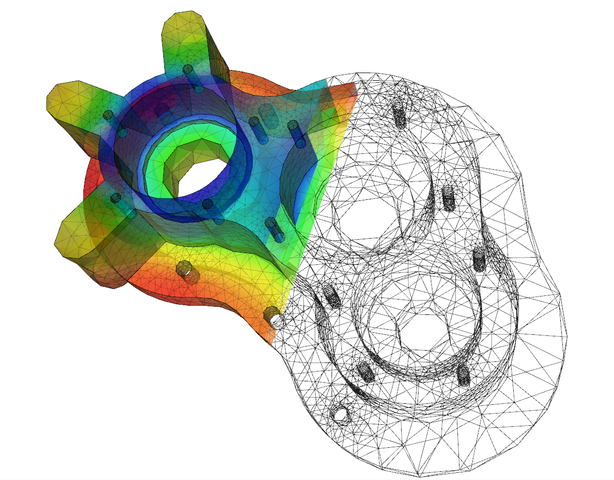
\includegraphics[scale=0.2]{imagenes/614px-Elmer-pump-heatequation.png} 
\caption{Ejemplo de uso de Elmer. \cite{ElmerpumpheatequationPng}}
 \label{fig:Elmer-pump-heatequation.png}
\end{figure}

\begin{figure} %con el [H] le obligamos a situar aquí la figura
\centering
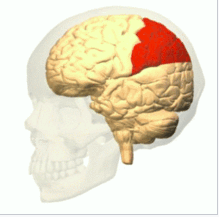
\includegraphics[scale=0.6]{imagenes/lobulo_parietal.png} 
\caption{Modelo 3D del Lobulo parietal, fuente Wikipedia} \label{fig:lobulo_parietal.png}
\end{figure}

\subsection{ Representaciones de Objectos}
Las dos representaciones tiene sus ventajas y desventajas. La representación de fronteras 
es una representación menos real y con más limitaciones en cuanto al cálculo de propiedades y estados del objeto pero permite una apariencia tan detallada como quieras con un menor coste de memoria del ordenador así como de tiempo de computo para la generación del objeto. Pero por otro lado tenemos la representación volumétrica que sí nos permite representar el objeto en su totalidad, es decir, incluyendo las capas que deseemos así como todas las propiedades de las distintas partes del interior del objeto. De esta forma es posible asignar distintos colores y transparencias a una cabeza humana para visualizar las partes que deseemos y tener una representación más fiel. Nuestro trabajo utiliza modelos de frontera, en concreto, mallas poligonales.\\

Otro apartado a tener en cuenta es forma de dibujar la malla. Pero primero es definir que es una malla, una malla poligonal. Una malla poligonal es un conjunto de vértices, aristas y caras, donde los vértices están unidos a través de aristas formando caras que a su vez forman una figura poligonal (ver ejemplo \ref{fig:mesh_overview.png}). Una de las características principales de una malla es la forma en la que se forman las caras dependiendo del número de aristas necesarias para formarlas. La forma más básica es el triángulo, que requiere la unión de tres vértices con tres aristas. La siguiente sería los \textit{quads} que requiere la unión de cuatro vértices con cuatro aristas. Y por último poligonal, que se compone de cinco o más vértices y el mismo número de aristas para formar una superficie. Cada forma tiene sus propiedades y requisitos, por ello la más utilizada sin entrar en muchos detalles es la forma más básica el triángulo ya que siempre está contenido en un plano. De hecho, el triángulo es el símplice 2D. Además permite una representación muy sencilla y rápida.\\

\begin{figure} %con el [H] le obligamos a situar aquí la figura
\centering
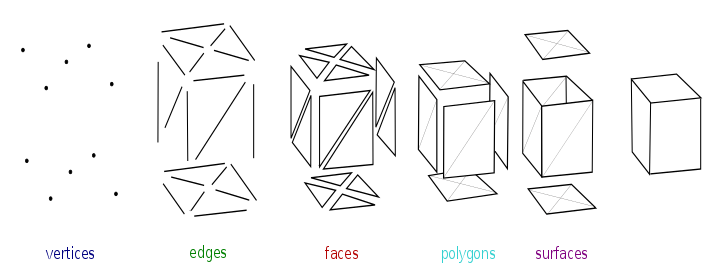
\includegraphics[scale=0.4]{imagenes/Mesh_overview.png} 
\caption{Partes de una malla poligonal, fuente Wikipedia (\cite{lobsterbakeEnglishLicensingCcbysa32009})} \label{fig:mesh_overview.png}
\end{figure}

Desde la definición de las mallas de triángulos se han investigado la forma de optimizar los recursos y acelerar los cálculo que se realizan sobre la misma. Algunas mejoras se centran en la forma de definir las aristas para la exploración y recorrido de la malla. Las mallas actuales con cierto grado de realismo cuentan fácilmente con varios miles de caras, que significa que requiere al menos tres veces más de vértices y de aristas, por esto es muy importante optimizar la forma en que se almacenan los datos y la forma de moverse por la malla. Una aproximación de movimiento por barrido, es decir, partiendo del primer vértice y luego al siguiente vértice para para ver si están conectados es una búsqueda exponencial del tipo $O(n^n)$ una búsqueda muy costosa.

La resolución de este problema derivó en la aparición de nuevas estructuras de datos para las aristas. Uno de los resultados fue las \textit{aristas aladas} una representación que guarda la información de donde procede la arista y a donde va, es decir, los dos vértices que delimitan la arista y de las aristas siguiente y anterior. Esta estructura optimiza la navegación por la malla pero tiene el inconveniente de que almacena dos veces cada arista, la que va del vértice $i$ al vértice $i+1$ y la que va del vértice $i+1$ al vértice $i$. De esté modo no es muy eficiente el almacenamiento de la estructura (ver figura \ref{fig:winger_edge.png}).\\ 


\begin{figure} %con el [H] le obligamos a situar aquí la figura
	\centering
	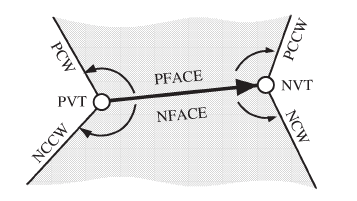
\includegraphics[scale=0.4]{imagenes/winger_edge.png} 
	\caption{Esquema de una arista alada, fuente (\cite{kettnerUsingGenericProgramming1999})} \label{fig:winger_edge.png}
\end{figure}


La siguiente solución que se dio a este problema fueron las \textit{''semi-aristas aladas``} definidas en (\cite{kettnerUsingGenericProgramming1999} y \cite{campagnaDirectedEdgesScalable1998} ) solucionan el problema del doble almacenamiento y además permiten un mayor conocimiento de la vecindad de la arista. Esta estructura supone que una arista está compuesta de dos semi-aristas una en cada dirección. Además se adjunta a cada semi-arista la información de la semi-arista siguiente, la anterior y la opuesta, entendiendo la opuesta como la semi-arista complementaria de la arista (ver figura \ref{fig:halfedge_small.png}). 

\begin{figure} %con el [H] le obligamos a situar aquí la figura
	\centering
	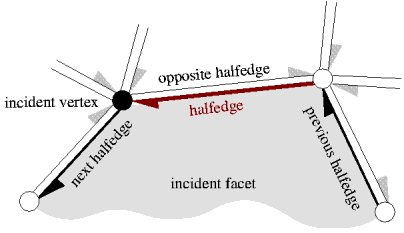
\includegraphics[scale=0.4]{imagenes/halfedge_small.png} 
	\caption{Esquema de una semi-arista alada, fuente The Computational Geometry Algorithms Library (\cite{CGAL12Halfedge})} \label{fig:halfedge_small.png}
\end{figure}

\subsection{APIs en informática gráfica}
En los años noventa la compañía \textit{``Silicon Graphics, Inc''} (SGI) desarrollaron la primera API para gráficos libre, OpenGL, del inglés Open Graphics Library \cite{OpenGLOverview}. SGI liberó una API potente para la época que facilitaba mucho la tarea del programador a la hora de programar todo el entorno de los gráficos. Rápidamente se estableció como la API de informática gráfica más usada, estableció algunos conceptos y formas de trabajar que se utilizan a día de hoy y que siguen inmutables y gran parte del software de gráficos utiliza directamente OpenGL o se basa en el. Un elemento fue la arquitectura de debían seguir para programar gráficos, además de establecer el cómo y que uso tiene del cauce gráfico. OpenGL ha ido sacando actualizaciones y mejoras sobre si mismo hasta llegar a la versión 4.5, pero su pensamiento base e ideas principales se mantienen.\\

En el año 2000 nació \textit{``Khronos Group''} (\cite{KhronosGroup2018}) una compañía para la cooperación y desarrollo del entorno virtual de la informática gráfica bajo los estándares abiertos. Se hicieron cargo de OpenGL y a partir de el desarrollaron más APIs para el desarrollo de gráficos, como fueron: \texttt{WebGL, OpenCL, SPIR, OpenVR, etc}. Entre ellas la más actual ha sido \texttt{Vulkan} una API que liberaron en febrero de 2016 para adaptar OpenGL al hardware moderno y actualizar su núcleo con las nuevas tecnologías. Las principales ventajas de \texttt{Vulkan} sobre \texttt{OpenGL} es que está pensado para aprovechar al máximo el hardware actual, en los años noventa casi todos o los más habituales eran los procesadores con un solo núcleo  y cauces muy lentos entre la tarjeta gráfica (GPU) apenas con memoria (\cite{NVIDIANV1}) y el procesador(CPU), por ello se destinaba casi todo el computo a la GPU y un poco de control en la CPU. \texttt{Vulkan} se sustenta en los procesadores de varios núcleos y cauces muy rápidos además de GPUs con arquitecturas superiores en cuanto paralelización y mucho mayor espacio de memoria. De esta forma \texttt{Vulkan} permite una paralelización muy superior a \texttt{OpenGL} entre otras ventajas.\\

\subsection{Objetivo del proyecto}
Este proyecto consta principalmente del procesado geométrico de una malla de triángulos. El procesado geométrico sobre una malla ofrece una gran versatilidad de operaciones sobre la malla tales como (Curso sobre procesado geométrico de la Universidad de Stanford \cite{mirelaben-chenCS468GeometryProcessing}):
simplificación de una malla, mejora de la calidad de una malla, deformaciones, mapeado de texturas, reconstrucciones de partes de la malla, detección de propiedades, etc. El campo del procesado geométrico es realmente amplio y con una infinidad de aplicaciones posibles.En este proyecto nos centramos en las operaciones más básicas pero muy importantes, como son la simplificación de una malla, voltear aristas cambiando así la topología de la malla (entre otras).

\subsubsection{Desarrollo de un Motor Gráfico}
Un apartado importante es el desarrollo de un motor gráfico que nos permita soportar mallas de triángulos. Este motor tiene que estar centrado en el procesado geométrico de las mallas y por tanto tiene que contener una una estructura de datos capaz de soportar dicha tarea. El procesado geométrico de mallas requiere de algoritmos de simplificación, modificación y operaciones de cálculo sobre la malla, estos algoritmos suelen ser bastante costosos en cuanto a recorrer la malla y aplicar operaciones por tanto la optimización de la estructura de datos y métodos aplicados debe ser muy eficiente. Para la estructura de datos se utilizará la estructura de semi-aristas aladas que proveen de una navegación por la malla eficaz y eficiente permitiendo así modificaciones más fáciles y de mejor eficiencia que otras estructuras \cite{kettnerUsingGenericProgramming1999}, obteniendo un buen resultado para el procesado geométrico.

\subsubsection{Visualizador de Mallas}
Otro aspecto del proyecto es la parte del visualizador de mallas o renderizador, cuya labor es generar la malla de triángulos en pantalla para que el usuario pueda verla. El visualizador se realizará utilizando las librerías de OpenGL y las tecnologías de QT que encapsulan el funcionamiento laborioso de OpenGL. El visualizador tiene que contar con operaciones básicas para el usuario como son el movimiento de la cámara por el espacio para poder visualizar como se deseé la malla y desde el angulo que prefiera.

\subsubsection{Procesamiento Geométrico}
Estudio e implementación de operaciones de procesamiento geométrico, en concreto de operaciones de simplificación de aristas y caras. Estas operaciones están enfocadas a mejorar la eficiencia de la malla mediante la reducción del número de aristas y de caras pero manteniendo siempre las propiedades de la malla, así como su forma en medida de lo posible.

Los algoritmos de simplificación son muy utilizados en las areas de ``Levels of details'' y optimización de escenas. Donde se debe de mantener un framerate, tasa de imagenes por segundo, sin que el usuario note el procesado. Estos algoritmos permiten la generación de escenas de películas y videojuegos cada vez más realistas manteniendo un consumo de recursos Hardware considerable.

\subsubsection{Decimation}
Todos los objetivos anteriores cada uno importante por si mismo deben juntarse para producir una API capaz de procesar el algoritmo de procesado geométrico \texttt{Decimation}, que dado un parámetro de tasa de reducción de triángulos especificado por le usuario aplique un algoritmo de simplificación de aristas y caras y lo muestre por la pantalla, a través de un visualizador de mallas. Por decirlo de algún modo es juntar todos los objetivos anteriormente descritos y construir un flujo de trabajo conjunto para un objetivo concreto. Aquí se probará la eficiencia y las operaciones implementadas en la estructura de datos.